\section{Mathematical Notation}
\label{reference_03}

Here we cover the complete mathematical notation of Event-B. For each expression (like an operator) we describe its purpose, its type, the type of its arguments and well-definedness-conditions. We roughly separate the expressions into three groups: predicates, set-theoretical and arithmetic.

Some laws (like the commutative law of addition in arithmetic) would be nice but will not be part of the first iteration of the documentation. E.g. the Z reference manual does this.

References to related proof rules would be nice to have, too. But again, this is not part of the first iteration.

\subsection{Introduction}

What data types exist, what are well-definedness-conditions, how the description of the expressions is organized.

\subsection{Predicates}

All operators that work with predicates ($\land$, $\lor$, quantifier, \ldots). 

\subsection{Sets and relations}

\subsubsection{Sets of functions}
\index{Function}\index{Injection}\index{Surjection}\index{Bijection}
\begin{rrnames}
  $\pfun$  & \texttt{+->}   & Partial functions\\
  $\tfun$  & \texttt{-->}   & Total functions \\
  $\pinj$  & \texttt{>+>}   & Partial injections\\
  $\tinj$  & \texttt{>->}   & Total injections \\
  $\psur$  & \texttt{+->>}  & Partial surjections\\
  $\tsur$  & \texttt{-->>}  & Total surjections \\
  $\tbij$  & \texttt{>->>}  & Bijections \\
\end{rrnames}
\begin{rodinrefentry}
  \rrdesc
  A partial function from $S$ to $T$ is a relation that maps an element of $S$ to at most one element
  of $T$. A function is total if its domain contains all elements of $S$, i.e. it maps every element
  of $S$ to an element of $T$.

  A function is injective (is an injection) if two distinct elements of $S$ are always mapped to distinct
  elements of $T$. An equivalent statement is that the inverse of the function is a also a function.

  A function is surjective (is a surjection) if for every element of $T$ there exists an element in $S$
  that is mapped to it.

  A function is bijective (is a bijection) if it is both injective and surjective.
  \rrdef
  $S \pfun T = \{~ f ~|~ f\in S\rel T \land (\forall e,x,y \qdot e\mapsto x\in f \land e\mapsto y\in f \limp x=y) ~\}$\\
  $S \tfun T = \{~ f ~|~ f\in S\pfun T \land \dom(f) = S ~\}$\\
  $S \pinj T = \{~ f ~|~ f\in S\pfun T \land f^{-1} \in  T\pfun S ~\}$\\
  $S \tinj T = (S\pinj T) \binter (S\tfun T)$\\
  $S \psur T = \{~ f ~|~ f\in S\pfun T \land \ran(f) = T ~\}$\\
  $S \tsur T = (S\psur T) \binter (S\tfun T)$\\
  $S \tbij T = (S\tinj T) \binter (S\tsur T)$\\
  \rrtypes
  With $S\in\pow(\alpha)$, $T\in\pow(\beta)$ and for each operator $\opelipse$ of $\pfun$, $\tfun$, $\pinj$, $\tinj$, $\psur$, $\tsur$, $\tbij$:\\
  $S \opelipse T \in \pow(\pow(\alpha\cprod\beta))$
  \rrwd
  For each operator $\opelipse$ of $\pfun$, $\tfun$, $\pinj$, $\tinj$, $\psur$, $\tsur$, $\tbij$:\\
  $\wdl(S\opelipse T) \defi \wdl(S) \land \wdl(T)$
\end{rodinrefentry}


\subsection{Arithmetic}

\subsubsection{Sets of numbers}
\begin{rrnames}
  $\intg$  & \texttt{INT}  & Integers \\
  $\nat$   & \texttt{NAT}  & Natural numbers, starting with 0 \\
  $\nat_1$ & \texttt{NAT1} & Natural numbers, starting with 1 \\
  $\upto$  & \texttt{..}   & Range of numbers
\end{rrnames}
\begin{rodinrefentry}
  \rrdesc
  The set of all integers is denoted by $\intg$. It contains all elements of the type.
  The two subsets $\nat$ and $\nat_1$ contain all elements greater or equal to 0 resp. 1.
  The range of numbers between $a$ and $b$ is denoted by $a \upto b$.
  \rrdef
  $\nat   = \{~ n ~|~ n\in\intg\land n\geq 0~\}$\\
  $\nat_1 = \{~ n ~|~ n\in\intg\land n\geq 1~\}$\\
  $a\upto b = \{~ n ~|~ n\in\intg\land a\leq n \land n\leq b~\}$
  \rrtypes
  $\intg\in\pow(\intg)$ \\
  $\nat\in \pow(\intg)$ \\
  $\nat_1\in\pow(\intg)$ \\
  $a \upto b\in\pow(\intg)$  with  $a\in\intg$ and $b\in\intg$
  \rrwd
  $\wdl(\intg) \defi \btrue$\\
  $\wdl(\nat) \defi \btrue$\\
  $\wdl(\nat_1) \defi \btrue$\\
  $\wdl(a \upto b) \defi \wdl(a) \land \wdl(b)$
\end{rodinrefentry}

\subsubsection{Arithmetic operations}
\begin{rrnames}
  $+$      & \texttt{+}   & Addition \\
  $-$      & \texttt{-}   & Subtraction or unary minus \\
  $\cdot$  & \texttt{*}   & Multiplication \\
  $\div$   & \texttt{/}   & Integer division \\
  $\bmod$  & \texttt{mod} & Modulo \\
\end{rrnames}
\begin{rodinrefentry}
  \rrdesc
  These are the usual arithmetic operations.
  \rrdef
    Addition, subtraction and multiplication behave as expected.

    The division is defined in a way that $1\div 2=0$ and $-1\div 2=0$:\\
    $a\div b = \max(\{~c ~|~ c\in\nat \land b\cdot c \leq a~\})$ for $a\in\nat$ and $b\in\nat$\\
%    $a\div b=c \defi \exists r \qdot 0\leq r \land r<b \land  b\cdot c + r = a$ for $a\in\nat$ and $b\in\nat$\\
    $(-a)\div b = - (a\div b)$\\
    $a\div (-b) = - (a\div b)$

    TODO: The same for modulo.
  \rrtypes
  With $a\in\intg$, $b\in\intg$ and for each operator $\opelipse$ of $+$, $-$, $\cdot$, $\div$, $\bmod$: \\
  $a\opelipse b\in\intg$\\
  $-a\in\intg$
  \rrwd
  $\wdl(a+b) \defi \wdl(a) \land \wdl(b)$ \\
  $\wdl(a-b) \defi \wdl(a) \land \wdl(b)$ \\
  $\wdl(-a) \defi \wdl(a)$ \\
  $\wdl(a\cdot b) \defi \wdl(a) \land \wdl(b)$ \\
  $\wdl(a\div b) \defi \wdl(a) \land \wdl(b) \land b\neq 0$ \\
  $\wdl(a\bmod b) \defi \wdl(a) \land \wdl(b) \land a\leq 0 \land b\neq 0$ \\
  TODO: Notation? $\wdl$ is actually implemented in Rodin. Is $\wdd$ still interesting?
  Or should we use something like the domain condition $\mathcal{DOM}$
  because it's simpler for operators?\\
\end{rodinrefentry}

\subsection{ASCII Representations of the Mathematical Symbols}
\label{ascii_representations_of_the_mathematical_symbols}

\marginpar{CONTENT MIGRATED FROM WIKI!}

The mathematical symbols used in the Event-B mathematical language are Unicode characters, beyond the ASCII subset. These characters are not always easy to input with a regular keyboard. To help users enter these characters, a list of standard input strings have been defined. When any of these strings is entered, it is automatically converted by the user interface to the corresponding Unicode character (i.e., mathematical symbol).

\subsubsection{Atomic Symbols}

\begin{center}
    \begin{tabular}{ | l | l | l | p{5cm} |}
    \hline
	ASCII & Symbol \\ \hline
	true & $\top$ \\ \hline
	false & $\bot$ \\ \hline
	INT & $\mathbb{Z}$ \\ \hline
	NAT & $\mathbb{N}$ \\ \hline
	NAT1 & $\mathbb{N_1}$ \\ \hline
    \end{tabular}
    \begin{tabular}{ | l | l | l | p{5cm} |}
    \hline
	ASCII & Symbol \\ \hline
	BOOL & $\mathrm{BOOL}$ \\ \hline
	TRUE & $\mathrm{TRUE}$ \\ \hline
	FALSE & $\mathrm{FALSE}$ \\ \hline
	\{\} & $\emptyset$ \\ \hline
    \end{tabular}
    \begin{tabular}{ | l | l | l | p{5cm} |}
    \hline
	ASCII & Symbol \\ \hline
	prj1 & $\prjone$ \\ \hline
	prj2 & $\prjtwo$ \\ \hline
	id & $\id$ \\ \hline
    \end{tabular}
\end{center}

\subsubsection{Unary Operators}

\begin{center}
    \begin{tabular}{ | l | l | l | p{5cm} |}
    \hline
	ASCII & Symbol \\ \hline
	not & $\neg$ \\ \hline
	finite & $finite$ \\ \hline
	card & $\card$ \\ \hline
	POW & $\pow$ \\ \hline
	POW1 & $\pown$ \\ \hline
    \end{tabular}
    \begin{tabular}{ | l | l | l | p{5cm} |}
    \hline
	ASCII & Symbol \\ \hline
	union & $\union$ \\ \hline
	inter & $\inter$ \\ \hline
	dom & $\dom$ \\ \hline
	ran & $\ran$ \\ \hline
%TODO: TILDE!
    \end{tabular}
    \begin{tabular}{ | l | l | l | p{5cm} |}
    \hline
	ASCII & Symbol \\ \hline
	min & $\min$ \\ \hline
	max & $\max$ \\ \hline
	- & $-$ \\ \hline
    \end{tabular}
\end{center}

\subsubsection{Assignment Operators}

\begin{center}
    \begin{tabular}{ | l | l | l | p{5cm} |}
    \hline
	ASCII & Symbol \\ \hline
	:= & $\bcmeq$ \\ \hline
	:| & $\bcmsuch$ \\ \hline
	:: & $\bcmin$ \\ \hline
    \end{tabular}
\end{center}

\subsubsection{Binary Operators}

\begin{center}
    \begin{tabular}{ | l | l | l | p{5cm} |}
    \hline
	ASCII & Symbol \\ \hline
	\& & $\land$ \\ \hline
	or & $\lor$ \\ \hline
	$=>$ & $\limp$ \\ \hline
	$<=>$ & $\leqv$ \\ \hline
	= & $=$ \\ \hline
	/= & $\neq$ \\ \hline
	: & $\in$ \\ \hline
	$<<:$ & $\subset$ \\ \hline
	$/<<:$ & $\not\subset$ \\ \hline
	$<:$ & $\subseteq$ \\ \hline
	$/<$: & $\not\subseteq$ \\ \hline
	$<$ & $<$ \\ \hline
	$<=$ & $\leq$ \\ \hline
	$>$ & $>$ \\ \hline
	$>=$ & $\geq$ \\ \hline
	/: & $\notin$ \\ \hline
    \end{tabular}
    \begin{tabular}{ | l | l | l | p{5cm} |}
    \hline
	ASCII & Symbol \\ \hline
	$|->$ & $\mapsto$ \\ \hline
	$<->$ & $\rel$ \\ \hline
	$<<->$ & $\trel$ \\ \hline
	$<->>$ & $\srel$ \\ \hline
	$<<->>$ & $\strel$ \\ \hline
	$+->$ & $\pfun$ \\ \hline
	$-->$ & $\tfun$ \\ \hline
	$+>>$ & $\psur$ \\ \hline
	$->>$ & $\tsur$ \\ \hline
	$>->>$ & $\tbij$ \\ \hline
	$/\backslash$ & $\binter$ \\ \hline
	$\backslash/$ & $\bunion$ \\ \hline
	$\backslash$ & $\setminus$ \\ \hline
	$**$ & $\cprod$ \\ \hline
	$>->$ & $\tinj$ \\ \hline
	$>+>$ & $\pinj$ \\ \hline
    \end{tabular}
    \begin{tabular}{ | l | l | l | p{5cm} |}
    \hline
	ASCII & Symbol \\ \hline
	$<+$ & $\ovl$ \\ \hline
	$||$ & $\pprod$ \\ \hline
	$><$ & $\dprod$ \\ \hline
	$circ$ & $\bcomp$ \\ \hline
	$;$ & $\fcomp$ \\ \hline
	$<|$ & $\domres$ \\ \hline
	$<<|$ & $\domsub$ \\ \hline
	$|>$ & $\ranres$ \\ \hline
	$-$ & $-$ \\ \hline
	$*$ & $*$ \\ \hline
	$/$ & $\div$ \\ \hline
	$..$ & $\upto$ \\ \hline
	$TODO$ & $\expn$ \\ \hline
	$+$ & $+$ \\ \hline
	$|>>$ & $\ransub$ \\ \hline
    \end{tabular}
    \begin{tabular}{ | l | l | l | p{5cm} |}
    \hline
	ASCII & Symbol \\ \hline
	$mod$ & $mod$ \\ \hline
    \end{tabular}
\end{center}

\subsubsection{Multiple Operators}

\begin{center}
    \begin{tabular}{ | l | l | l | p{5cm} |}
    \hline
	ASCII & Symbol \\ \hline
	partition & $partition$ \\ \hline
    \end{tabular}
\end{center}

\subsubsection{Quantifiers}

\begin{center}
    \begin{tabular}{ | l | l | l | p{5cm} |}
    \hline
	ASCII & Symbol \\ \hline
	! & $\forall$ \\ \hline
	\# & $\exists$ \\ \hline
	\% & $\lambda$ \\ \hline
	UNION & $\Union$ \\ \hline
	INTER & $\Inter$ \\ \hline
	| & $|$ \\ \hline
	. & $\qdot$ \\ \hline
    \end{tabular}
\end{center}

\subsubsection{Bracketing}

\begin{center}
    \begin{tabular}{ | l | l | l | p{5cm} |}
    \hline
	ASCII & Symbol \\ \hline
	oftype & $\forall$ \\ \hline
	\# & $\exists$ \\ \hline
	\% & $\lambda$ \\ \hline
	UNION & $\Union$ \\ \hline
	INTER & $\Inter$ \\ \hline
	| & $|$ \\ \hline
	. & $\qdot$ \\ \hline
    \end{tabular}
\end{center}

\begin{center}
    \begin{tabular}{ | l | l | l | p{5cm} |}
    \hline
	ASCII & Symbol \\ \hline
	( & $($ \\ \hline
	) & $)$ \\ \hline
	[ & $[$ \\ \hline
	] & $]$ \\ \hline
	\{ & $\{$ \\ \hline
	\} & $\}$ \\ \hline
    \end{tabular}
\end{center}

\subsubsection{Typing}

\begin{center}
    \begin{tabular}{ | l | l | l | p{5cm} |}
    \hline
	ASCII & Symbol \\ \hline
	oftype & 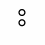
\includegraphics[]{img/reference/ref_03_offtype_symbol.png} \\ \hline
    \end{tabular}
\end{center}

%%% Local Variables: 
%%% mode: latex
%%% TeX-master: "rodin-doc"
%%% End: 
